\begin{enumerate}[label=\bfseries Câu \arabic*:]
	\item \mkstar{1}
	
\cauhoi{
	
	Nhận xét nào sau đây về biên độ dao động tổng hợp là \textbf{không} đúng? Dao động tổng hợp của hai dao động điều hòa cùng phương, cùng tần số
	\begin{mcq}
		\item có biên độ phụ thuộc vào biên độ của dao động hợp thành thứ nhất.
		\item có biên độ phụ thuộc vào tần số chung của hai dao động hợp thành.
		\item có biên độ phụ thuộc vào biên độ của dao động hợp thành thứ hai.
		\item có biên độ phụ thuộc vào độ lệch pha giữa hai dao động hợp thành.
	\end{mcq}
}
\loigiai{
	\textbf{Đáp án B.}
	
	Dao động tổng hợp của hai dao động điều hòa cùng phương, cùng tần số có biên độ phụ thuộc vào biên độ của dao động hợp thành thứ nhất, dao động hợp thành thứ hai, và pha dao động.
}
\item \mkstar{1}

\cauhoi{
	
	Xét dao động tổng hợp của hai dao động thành phần có cùng phương và cùng tần số. Biên độ của dao động tổng hợp \textbf{không} phụ thuộc vào
	\begin{mcq}
		\item tần số chung của hai dao động thành phần.
		\item biên độ của dao động thành phần thứ nhất.
		\item biên độ của dao động thành phần thứ hai.
		\item độ lệch pha của hai dao động thành phần.
	\end{mcq}
}
\loigiai{
	\textbf{Đáp án A.}
	
	Xét dao động tổng hợp cuả hai dao động thành phần có cùng phương và cùng tần số. Biên độ của dao động tổng hợp không phụ thuộc tần số chung của hai dao động thành phần.
	
}
\item \mkstar{2}

\cauhoi{
	
	Một vật thực hiện đồng thời hai dao động điều hòa $x_1 =3\cos \left(4\pi t +\dfrac{\pi}{6}\right)\ \text{cm}$ và $x_2 =3\cos \left(4\pi t + \dfrac{\pi}{2}\right)\ \text{cm}$. Hãy xác định dao động tổng hợp của hai dao động trên.
	\begin{mcq}(2)
		\item $x=3\sqrt 3\cos \left(4\pi t + \dfrac{\pi}{6}\right)\ \text{cm}$.
		\item $x=3\sqrt 3\cos \left(4\pi t + \dfrac{\pi}{3}\right)\ \text{cm}$.
		\item $x=3\cos \left(4\pi t + \dfrac{\pi}{6}\right)\ \text{cm}$.
		\item $x=3\cos \left(4\pi t - \dfrac{\pi}{6}\right)\ \text{cm}$.
	\end{mcq}
}
\loigiai{
	\textbf{Đáp án B.}
	
	Ta có dao động tổng hợp có dạng $x=A\cos(\omega t+\varphi)\ \text{cm}$.
	
	Trong đó:
	$A = \sqrt {A^2_1+A^2_2+2A_1A_2\cos (\varphi_2-\varphi_1)} = 3\sqrt 3\ \text{cm}$.
	
	$\tan \varphi =\dfrac{A_1\sin \varphi_1 + A_2\sin \varphi_2}{A_1 \cos \varphi_1 + A_2 \cos \varphi_2}= \sqrt 3 \Rightarrow \varphi =\dfrac{\pi}{3}$.
	
	Phương trình dao động cần tìm $x=3\sqrt 3\cos \left(4\pi t +\dfrac{\pi}{3}\right)\ \text{cm}$.
}
\item \mkstar{2}

\cauhoi{ 
	
	Một vật thực hiện đồng thời hai dao động điều hòa với biên độ lần lượt là 3 cm và 5 cm. Trong các giá trị sau giá trị nào \textbf{không} thể là biên độ của dao động tổng hợp?
	
	\begin{mcq}(4)
		\item 4 cm.
		\item 5 cm.
		\item 3 cm.
		\item 10 cm.
	\end{mcq}
}
\loigiai{
	\textbf{Đáp án D.}
	
	Ta có $|A_1-A_2| \leq A \leq A_1+A_2$.
	
	$\Rightarrow 2\ \text{cm} \leq A \leq 8\ \text{cm}$.
	
}
\item \mkstar{2}

\cauhoi{
	
	Dao động của một chất điểm có khối lượng 100 g là tổng hợp của hai dao động điều hòa cùng phương, có phương trình li độ lần lượt là $x_1 = 5\cos(10t)$ và $x_2 = 10\cos(10t)$ ($x_1$ và $x_2$ tính bằng cm, $t$ tính bằng s). Mốc thế năng ở vị trí cân bằng. Cơ năng của chất điểm bằng
	\begin{mcq}(4)
		\item 0,1125 J.
		\item 225 J.
		\item 112,5 J.		
		\item 0,225 J.
	\end{mcq}
	
}
\loigiai{
	\textbf{Đáp án A.}
	
	Hai dao động trên cùng pha vì thế biên độ dao động tổng hợp: $A = A_1+A_2 =\SI{15}{cm}$.
	
	Cơ năng của chất điểm: $W=\dfrac{1}{2} m \omega^2 A^2=\SI{0,1125}{J}$.
}
\item \mkstar{3}

\cauhoi{
	
	Tiến hành thí nghiệm do gia tốc trọng trường bằng con lắc đơn, một học sinh đo được chiều dài con lắc là $(119 \pm 1)\ \text{m/s}^2$. Chu kì dao động nhỏ của nó là $(\text{2,20} \pm \text{0,01}\ \text{s})$. Lấy $\pi^2 =\text{9,87}$ và bỏ qua sai số của số $\pi$. Gia tốc trọng trường do học sinh đo được tại nơi làm thí nghiệm là
	\begin{mcq}(2)
		\item $g= (\text{9,7} \pm \text{0,1})\ \text{m/s}^2$.
		\item $g= (\text{9,8} \pm \text{0,1})\ \text{m/s}^2$.
		\item $g= (\text{9,7} \pm \text{0,2})\ \text{m/s}^2$.			
		\item $g= (\text{9,8} \pm \text{0,2})\ \text{m/s}^2$.
	\end{mcq}
	
}
\loigiai{
	\textbf{Đáp án C.}
	
	Áp dụng công thức: 
	
	$\overline{T} =2\pi \sqrt {\dfrac{\overline{l}}{\overline{g}}} \Rightarrow \overline{g} =\dfrac{4 \pi^2 \overline{l}}{\overline{T}^2}=\text{9,706}=\text{9,7}\ \text{m/s}^2$.
	
	Sai số tương đối ($\varepsilon$):
	
	$\varepsilon =\dfrac{\Delta g}{\overline{g}} =\dfrac{\Delta l}{l}+2\dfrac{\Delta T}{T} =\text{0,0175} \Rightarrow \Delta g = \overline{g} \varepsilon = \text{0,2}.$
	
	Gia tốc $g = \overline {g}+\Delta g = g= (\text{9,7} \pm \text{0,2})\ \text{m/s}^2$.
}
\item \mkstar{3}

\cauhoi{
	
	Một chất điểm tham gia đồng thời hai dao động điều hòa cùng tần số trên trục Ox. Biết dao động thành phần thứ nhất có biên độ $A_1=4\sqrt{3}\ \text{cm}$, dao động tổng hợp có biên độ $A=\SI{4}{cm}$. Dao động thành phần thứ hai sớm pha hơn dao động tổng hợp và $\dfrac{\pi}{3}$. Dao động thành phần thứ hai có biên độ là
	\begin{mcq}(4)
		\item $6\sqrt{3}\ \text{cm}$
		\item $4\sqrt{3}\ \text{cm}$.
		\item $8\ \text{cm}$.		
		\item $4\ \text{cm}$.
	\end{mcq}
	
}
\loigiai{
	\textbf{Đáp án C.}
	
	Xác định biên độ của dao động thành phần thứ nhất: 
	
	$A_1^2=A^2+A_2^2$ $-2\cdot A \cdot A_2\cos(\varphi_2-\varphi)$.
	
	Thay số vào ta có: 
	
	$(4\sqrt{3})^2=4^2+A_2^2-2\cdot 4\cdot A_2\cos(\dfrac{\pi}{3})$. 
	
	$\Rightarrow A_2^2-4\cdot A_2-32=0$.
	
	$  \Rightarrow A_2=8\ \text{cm}$.
	
	
	
}

\item \mkstar{3}

\cauhoi{
	
	Một vật khối lượng 100 g tham gia đồng thời hai dao động cùng phương, cùng tần số góc 10 rad/s, biên độ $A_1$ và $A_2$ với $\dfrac{A_1}{A_2}=\sqrt{3}$ và vuông pha với nhau. Động năng của vật có giá trị cực đại là 50 mJ. Giá trị $A_2$ là
	\begin{mcq}(4)
		\item 5 cm.
		\item 0,5 m.
		\item 6 cm.
		\item 25 cm.
	\end{mcq}
	
}
\loigiai{
	\textbf{Đáp án A.}
	
	Hai dao động vuông pha $A^2=A_1^2+A_2^2$ (1).
	
	Theo đề bài ta có $A_1=\sqrt{3}A_2$ (2).
	
	Ta lại có: $W_\text{đmax}=W=\dfrac{1}{2}m\omega^2A^2 \Rightarrow A$(3).
	
	Thay(3) và (2) vào (1) suy ra $A_2$.
	
	
	
}
\item \mkstar{2}

\cauhoi{
	
	Chuyển động của vật là tổng hợp của hai dao động điều hòa cùng phương. Hai dao động này có phương trình lần lượt là: $x_1=4\cos\left(10t+\dfrac{\pi}{4}\right)\ \text{cm}$ và $x_2=3\cos(10t-\dfrac{3\pi}{4})\ \text{cm}$. Độ lớn vận tốc của vật ở vị trí cân bằng là
	\begin{mcq}(4)
		\item 100 cm/s.
		\item 10 cm/s.
		\item 50 cm/s.
		\item 80 cm/s.
	\end{mcq}
	
}
\loigiai{
	\textbf{Đáp án A.}
	
	Dao động tổng hợp $x=A\cos(10t+\varphi)$. 
	
	Hai dao động ngược pha $A=A_1-A_2 \Rightarrow$ $v_\text{max}=\omega A$
	
	
	
}

\item \mkstar{2}

\cauhoi{
	
	Cho hai dao động điều hoà: $x_1 = A_1\cos\left(\omega t+\dfrac{\pi}{6}\right)$, $x_2 = A_2\cos\left(\omega t-\dfrac{5\pi}{6}\right)$. Hai dao động trên: 
	\begin{mcq}(2)
		\item lệch pha nhau $\dfrac{2\pi}{3}$.
		\item cùng pha.
		\item ngược pha.
		\item lệch pha nhau $\dfrac{\pi}{2}$.
	\end{mcq}
	
}
\loigiai{
	\textbf{Đáp án C.}
	
	$\Delta \varphi = \pi $ nên hai dao động trên ngược pha.
	
	
	
}
		\item \mkstar{3}
		
	\cauhoi{
		
		Hai chất điểm M và N có cùng khối lượng, dao động điều hòa cùng tần số góc theo hai đường thẳng song song kề nhau và song song với trục tọa độ Ox. Vị trí cân bằng của M và của N đều ở trên một đường thẳng qua gốc tọa độ và vuông góc với Ox. Biên độ của M là $6\ \text{cm}$, của N là $8\ \text{cm}$. Trong quá trình dao động, khoảng cách lớn nhất giữa M và N theo phương Ox là $10\ \text{cm}$. Mốc thế năng tại vị trí cân bằng. Ở thời điểm mà M có động năng bằng thế năng, tỉ số động năng của M và động năng của N là
		\begin{mcq}(4)
			\item $\dfrac{16}{9}$.
			\item $\dfrac{9}{16}$.
			\item $\dfrac{3}{4}$.
			\item $\dfrac{4}{3}$.
		\end{mcq}
	}
	\loigiai{
		\textbf{Đáp án B.}
		
		\begin{center}
			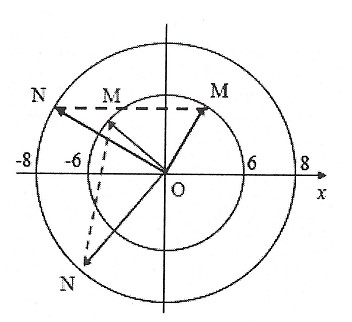
\includegraphics[scale=0.8]{../figs/VN12-PH-06-P-005-1-h1.jpg}
		\end{center}
		
		
		Khoảng cách giữa M và N là $\Delta x=\left| x_M-x_N \right|=\left|6\cos \left(\omega t+\varphi_1 \right)-  8\cos \left(\omega t+\varphi_2 \right) \right| =A\left|\cos \left( \omega t+\varphi \right)  \right|  $.
		
		Khoảng cách lớn nhất khi MN có phương nằm ngang, suy ra $6^2+8^2=10^2$, suy ra OM  luôn vuông góc với ON.
		
		Ở thời điểm mà M có động năng bằng thế năng tại: $x_M=A\dfrac{\sqrt{2}}{2}\left( W_\text{đM}= W_\text{tM}=\dfrac{1}{2}W_M \right) $.
		
		Tức OM hợp với Ox góc $\dfrac{\pi}{4}$, suy ra ON hợp với Ox góc $\dfrac{\pi}{4}$ hay  $x_N=-A\dfrac{\sqrt{2}}{2}$.
		
		Suy ra $W_\text{đN}=W_\text{tN}=\dfrac{1}{2}W_N$.
		
		Do đó, $\dfrac{W_\text{tM}}{W_\text{tN}}=\dfrac{W_\text{M}}{W_\text{N}}=\dfrac{9}{16}$.
		
		
	}
	\item \mkstar{3}
	
	\cauhoi{
		
		Hai chất điểm dao động điều hòa cùng tần số, trên hai đường thẳng song song với nhau và song song với trục Ox có phương trình lần lượt là $x_1=A_1\cos \left(\omega t+\varphi_1 \right)$   và $x_2=A_2\cos \left(\omega t+\varphi_2 \right)$. Giả sử $x=x_1+x_2$   và $y=x_1-x_2$. Biết rằng biên độ dao động của $x$ gấp $2$ lần biên độ dao động của $y$. Độ lệch pha giữa $x_1$ và $x_2$ là $\Delta \varphi$. Giá trị nhỏ nhất của  $\cos \Delta \varphi$ là
		\begin{mcq}(4)
			\item $\text{0,5}$.
			\item $\text{0,25}$.
			\item $-1$.
			\item $\text{0,6}$.
		\end{mcq}
	}
	\loigiai{
		\textbf{Đáp án D.}
		
		Ta có: $A_x^2=A_1^2+A_2^2+2A_1A_2\cos \Delta \varphi=4A_Y^2$ và $A_y^2=A_1^2+A_2^2-2A_1A_2\cos \Delta \varphi$.
		
		Suy ra: $4A_1A_2\cos \Delta \varphi =3A_y^2$ và $5A_y^2=2\left( A_1^2+A_2^2\right)$.
		
		Suy ra $\cos \Delta \varphi=\dfrac{3}{10}\cdot \dfrac{A_1^2+A_2^2}{A_1A_2}\geq \dfrac{3}{10} \cdot \dfrac{2A_1A_2}{A_1A_2}= \text{0,6}$.
		
		
	}
	\item \mkstar{3}

\cauhoi{
	
	Một chất điểm dao động điều hòa có đồ thi biểu diễn sự phụ thuộc của li độ $x$ vào thời gian $t$ như hình vẽ. Tại thời điểm $t = \text{0,2}\ \text{s}$, chất có li độ $2\ \text{cm}$. Ở thời điểm $t = \text{0,9}\ \text{s}$, gia tốc của chất điểm có giá trị bằng
	\begin{center}
		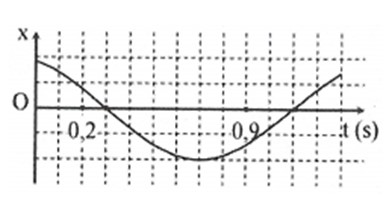
\includegraphics[scale=0.8]{../figs/VN12-PH-06-P-005-1-h7.jpg}
	\end{center}
	
	\begin{mcq}(4)
		\item $\text{14,5}\ \text{cm/s}^2$.
		\item $\text{57,0}\ \text{cm/s}^2$.
		\item $\text{5,7}\ \text{m/s}^2$.		
		\item $\text{1,45}\ \text{m/s}^2$.
	\end{mcq}
	
}
\loigiai{
	\textbf{Đáp án B.}
	
	Áp dụng công thức: 
	
	Dựa vào đồ thị ta thấy mỗi ô vuông ứng với thời gian là $\text{0,1}\ \text{s}$.
	
	Khoảng thời gian $2$ lần liên tiếp vật có li độ $x=0$ là (ứng với 8 ô)
	
	Tại thời điểm $t = \text{0,3}\ \text{s}$ ta có: $x=0\ \text{cm}, \ v<0$, suy ra $\varphi_3=\dfrac{\pi}{2}$.
	
	Pha dao động tại thời điểm $t = \text{0,2}\ \text{s}$ là $\varphi_2=\varphi_3-\dfrac{5\pi}{4}\cdot \text{0,1}=\dfrac{3\pi}{8}$.
	
	Do đó $A\cos \dfrac{3\pi}{8}=2\Rightarrow A=\text{5,226}\ \text{cm}$.
	
	Mặt khác $\Delta t=t_{0,2\rightarrow 0,9}=\text{0,7}\ \text{s}\Rightarrow \Delta \varphi=\text{0,7}\cdot \dfrac{5\pi}{4}=\dfrac{7\pi}{8}$.
	
	Do đó $x_{t=0,9}=A\cos \left(\dfrac{3\pi}{8}+\dfrac{7\pi}{8} \right)=-\text{3,696}\ \text{cm}\Rightarrow a=-\omega^2 x=57\ \text{cm/s}^2$.
	
}
\item \mkstar{3}

\cauhoi{
	
	Hình vẽ là đồ thị biểu diễn độ dời của dao động $x$ theo thời gian $t$ của một vật dao động điều hòa. Phương trình dao động của vật là
	\begin{center}
		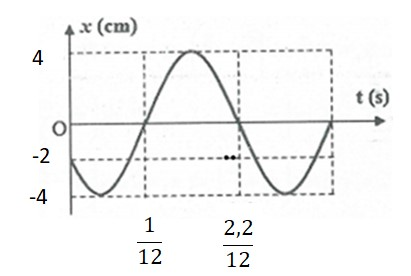
\includegraphics[scale=0.8]{../figs/VN12-PH-06-P-005-1-h6.jpg}
	\end{center}
	
	\begin{mcq}(2)
		\item $x=4\cos \left( 10\pi t+\dfrac{2\pi}{3}\right)\ \text{cm}$.
		\item  $x=4\cos \left( 20\pi t+\dfrac{2\pi}{3}\right)\ \text{cm}$.
		\item  $x=4\cos \left( 10\pi t+\dfrac{5\pi}{6}\right)\ \text{cm}$.	
		\item  $x=4\cos \left( 20\pi t-\dfrac{\pi}{3}\right)\ \text{cm}$.
	\end{mcq}
	
}
\loigiai{
	\textbf{Đáp án A.}
	
	Ta có  $A=4\ \text{cm}, \ \dfrac{T}{2}=\dfrac{\text{2,2}-1}{12}\Rightarrow T=\dfrac{1}{5}\ \text{s}\Rightarrow \omega =10\pi$.
	
	Tại thời điểm $t = 0$ ta có: $x=-2=-\dfrac{A}{2}, \ v<0$, suy ra $\varphi_0=\dfrac{2\pi}{3}$.
	
}

\item \mkstar{3}

\cauhoi{
	
	Đồ thị dao động của một chất điểm dao động điều hòa như hình vẽ. Phương trình biểu diễn sự phụ thuộc của vận tốc của vật theo thời gian là
	
	\begin{center}
		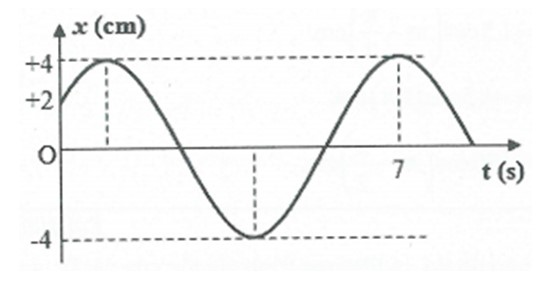
\includegraphics[scale=0.8]{../figs/VN12-PH-06-P-005-1-h8.jpg}
	\end{center}
	\begin{mcq}(2)
		\item $v=\dfrac{4\pi}{3} \cos \left( \dfrac{\pi}{3} t+\dfrac{\pi}{6}\right)\ \text{cm/s} $.
		\item $v=\dfrac{4\pi}{3} \cos \left( \dfrac{\pi}{6} t+\dfrac{5\pi}{6}\right)\ \text{cm/s} $.
		\item $v=4\pi \cos \left( \dfrac{\pi}{3} t+\dfrac{\pi}{3}\right)\ \text{cm/s} $.
		\item $v=4\pi \cos \left( \dfrac{\pi}{6} t+\dfrac{\pi}{3}\right)\ \text{cm/s} $.
	\end{mcq}
	
}
\loigiai{
	\textbf{Đáp án A.}
	
	Dựa vào đồ thị ta thấy: tại thời điểm $t=0$, suy ra $x=2, \ v>0\Rightarrow \varphi_0=-\dfrac{\pi}{3}$.
	
	Lại có: $t_{2 \rightarrow 4}+T=7\Rightarrow T=6\ \text{s}\Rightarrow \omega=\dfrac{\pi}{3}\ \text{rad/s}$.
	
	Do đó $x=4\cos \left( \dfrac{\pi t}{3}-\dfrac{\pi}{3}\right)\ \text{cm}\Rightarrow v=\dfrac{4\pi}{3}\cos \left( \dfrac{\pi t}{3}+\dfrac{\pi}{6}\right)\ \text{cm/s}$. 
	
	
	
}
\item \mkstar{3}

\cauhoi{
	
	Cho hai dao dộng cùng phương có phương trình $x_1=A_1\cos \left(\omega t+ \varphi_1 \right) $  và  $x_2=A_1\cos \left(\omega t + \varphi_2 \right) $  ($x$ tính bằng cm, $t$ được tính bằng s). Đồ thị dao động tổng hợp $x=x_1+x_2$ có dạng như hình vẽ. Cặp phương trình $x_1, \ x_2 $ nào sau đây thỏa mãn với đồ thị?
	\begin{center}
		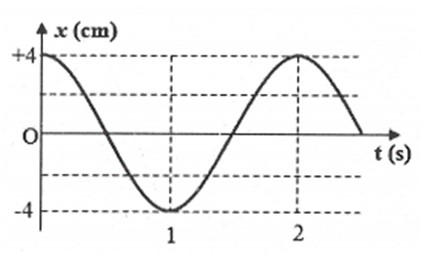
\includegraphics[scale=0.8]{../figs/VN12-PH-06-P-005-1-h9.jpg}
	\end{center}
	
	\begin{mcq}
		\item $x_1=2\sqrt{2}\cos \left( \pi t-\dfrac{\pi}{4}\right)\ \text{cm}$ và $x_2=2\sqrt{2}\cos \left( \pi t+\dfrac{\pi}{4}\right)\ \text{cm}$.
		\item $x_1=2\cos \left( \pi t-\dfrac{\pi}{2}\right)\ \text{cm}$ và $x_2=2\cos \left( \pi t+\dfrac{\pi}{2}\right)\ \text{cm}$.
		\item $x_1=6\cos \left( \pi t+\dfrac{\pi}{2}\right)\ \text{cm}$ và $x_2=2\cos \left( \pi t-\dfrac{\pi}{2}\right)\ \text{cm}$.
		\item $x_1=4\cos \left( \pi t+\dfrac{\pi}{3}\right)\ \text{cm}$ và $x_2=4\cos \left( \pi t-\dfrac{\pi}{3}\right)\ \text{cm}$.
	\end{mcq}
	
}
\loigiai{
	\textbf{Đáp án D.}
	
	Dựa vào đồ thị ta có: $A=4\ \text{cm}, \ \dfrac{T}{2}=1\ \text{s}\Rightarrow T=2\ \text{s}\Rightarrow \omega =\pi\ \text{rad/s}$.
	
	Tại thời điểm $t=0\Rightarrow x=A\Rightarrow \varphi=0$.
	
	Do đó  $x=x_1+x_2=4\cos \pi t=4\cos \left( \pi t+\dfrac{\pi}{3}\right)+ 4\cos \left( \pi t-\dfrac{\pi}{3}\right)$.
	
	
	
	
}

\item \mkstar{3}

\cauhoi{ 
	
	Một chất điểm dao động điều hòa dọc theo trục Ox, với O  trùng với vị trí cân bằng của chất điểm. Đường biểu diễn sự phụ thuộc li độ chất điểm theo thời gian $t$ cho ở hình vẽ. Phương trình vận tốc của chất điểm là
	\begin{center}
		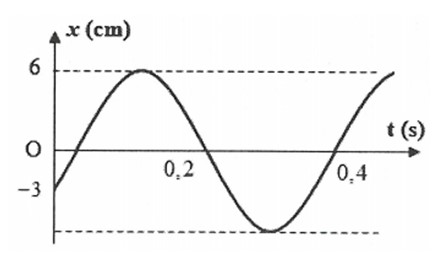
\includegraphics[scale=0.8]{../figs/VN12-PH-06-P-005-1-H5.jpg}
	\end{center}
	
	
	\begin{mcq}(2)
		\item $v=60\pi \cos \left( 5\pi t-\dfrac{\pi}{3}\right) $.
		\item $v=60\pi \cos \left( 5\pi t-\dfrac{\pi}{6}\right) $.
		\item $v=60\cos \left( 5\pi t-\dfrac{\pi}{3}\right) $.
		\item $v=60\pi \cos \left( 5\pi t-\dfrac{\pi}{6}\right) $.
	\end{mcq}
	
}
\loigiai{
	\textbf{Đáp án B.}
	
	
	
	Biên độ doa động của vật là $A = 6\ \text{cm}$.
	
	Dựa vào đồ thị ta thấy rằng sau $\text{0,2}\ \text{s}$ trạng thái dao động vật được lặp lại, do đó  $T=\text{0,2}\ \text{s}\Rightarrow  \omega=\dfrac{2\pi}{T}=5\pi \ \text{rad/s}$.
	
	Tại thời điểm bạn đầu $x=-3\ \text{cm}=-\dfrac{A}{2}$ và $v>0$, suy ra $\varphi_0=-\dfrac{2\pi}{3}$.
	
	
	Do đó phương trình dao động của vật là $x=6\cos \left(5\pi t-\dfrac{2\pi}{3}\right)\ \text{cm}$.
	
	Suy ra $v=60\pi \cos \left( 10\pi t-\dfrac{2\pi}{3}+\dfrac{\pi}{2}\right)= 60\pi \cos \left( 10\pi t-\dfrac{\pi}{6}\right) $.
	
	
	
	
	
}
	\item \mkstar{4}
	
	\cauhoi{
		
		Cho $D_1, \ D_2$ và $D_3$ là ba dao động điều hòa cùng phương, cùng tần số. Dao động tổng hợp của $D_1$   và $D_2$  có phương trình là $x_{12}=3\sqrt{3}\cos \left( \omega t+\dfrac{\pi}{2}\right) $  cm. Dao động tổng hợp của $D_2$   và $D_3$   có phương trình  $x_{23}=3\cos \left( \omega t\right) $  cm. Dao động $D_1$   ngược pha với dao động $D_3$. Biên độ dao động $D_2$  có giá trị nhỏ nhất là
		
		\begin{mcq}(4)
			\item $\text{2,6}\ \text{cm}$.
			\item $\text{2,7}\ \text{cm}$.
			\item $\text{3,6}\ \text{cm}$.
			\item $\text{3,7}\ \text{cm}$.
		\end{mcq}
	}
	\loigiai{
		\textbf{Đáp án A.}
		
		Ta có: $x_1+x_2=x_\text{12}=3\sqrt{3}\cos \left( \omega t+\dfrac{\pi}{2}\right)$   và  $x_{23}=x_2+x_3=3\cos \left( \omega t\right) $  cm.
		
		Suy ra $x_1-x_3=3\sqrt{3}\angle \dfrac{\pi}{2}-3\angle 0=6\angle \dfrac{2\pi}{3}$.
		
		Do dao động $D_1$ ngược pha với dao động $D_3$ nên   $x_3=-kx_1\Rightarrow x_1=\dfrac{6}{k+1}\angle \dfrac{2\pi}{3}$ với $k>0$.
		
		Do đó $x_2=3\sqrt{3}\angle \dfrac{\pi}{2}-\dfrac{6}{k+1}\angle \dfrac{2\pi}{3}\ (k>0) $.
		
		Suy ra $A_2^2=(3\sqrt{3})^2+\left( \dfrac{6}{k+1}\right)^2-2\cdot 3\sqrt{3}\cdot \dfrac{6}{k+1}\cdot \cos \dfrac{\pi}{6}=27+t^2-9t\ (t=\dfrac{6}{k+1}) $.
		
		Vậy $A_2^2=\left(t-\dfrac{9}{2} \right)^2+\dfrac{27}{4}\geq \dfrac{27}{4}\Rightarrow A_2\geq \dfrac{3\sqrt{3}}{2}=\text{2,6}\ \text{cm} $.
		
		Dấu bằng xảy ra khi $\dfrac{6}{k+1}=\dfrac{9}{2}\Rightarrow k=\dfrac{1}{3}\ \text{thỏa mãn}$. 
		
		
	}
	\item \mkstar{4}
	
	\cauhoi{ 
		
		Điểm sáng A đặt trên trục chính của một thấu kính, cách thấu kính $10\ \text{cm}$. Chọn trục tọa độ Ox vuông góc với trục chính, gốc O nằm trên trục chính của thấu kính. Cho A dao động điều hòa theo phương của trục Ox. Biết phương trình dao động của A là $x$ và ảnh $A'$  là $x'$  của nó qua thấu kính được biểu diễn như hình vẽ. Thời điểm lần thứ $2018$ mà khoảng cách giữa vật sáng và ảnh của nó khi điểm sáng A dao động là $5\sqrt{5}\ \text{cm}$ có giá trị gần bằng giá trị nào sau đây nhất?
		\begin{center}
			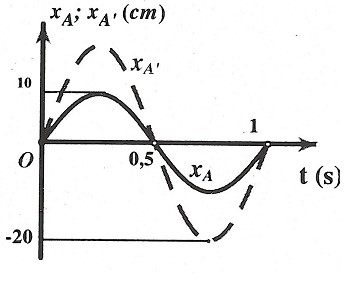
\includegraphics[scale=0.8]{../figs/VN12-PH-06-P-005-1-h2.jpg}
		\end{center}	
		\begin{mcq}(4)
			\item $\text{504,6}\ \text{s}$.
			\item $\text{506,8}\ \text{s}$.
			\item $\text{506,4}\ \text{s}$.
			\item $\text{504,2}\ \text{s}$.
		\end{mcq}
	}
	\loigiai{
		\textbf{Đáp án D.}
		
		\begin{center}
			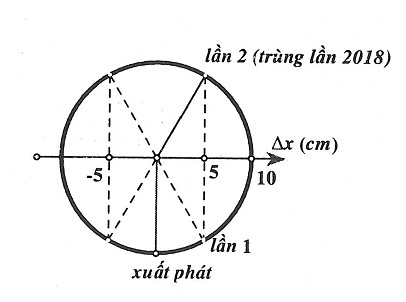
\includegraphics[scale=0.8]{../figs/VN12-PH-06-P-005-1-h3.jpg}
		\end{center}
		
		Từ đồ thị ta được: ảnh nhỏ hơn vật và cùng tính chất với vật, suy ra đây là thấu kính hội tụ,  $k = 2$.
		
		Áp dụng $k=\dfrac{f}{f-d}\Rightarrow f=20\ \text{cm}$, suy ra $d'=\dfrac{df}{d-f}=-20\ \text{cm}$.
		
		Khoảng cách vật và ảnh: $\Delta d=|d+d'|=10\ \text{cm}$.
		
		Từ đồ thị ta cũng viết được: $x_A=10\cos \left(\omega t-\dfrac{\pi}{2} \right) \ \text{cm} $ và $x_A'=20\cos \left(\omega t-\dfrac{\pi}{2} \right)\ \text{cm}$.
		
		Phương trình khoảng cách ảnh và vật trên phương Ox:
		$\Delta x=x_A-x_A'=10\cos \left( \omega t -\dfrac{\pi}{2}\right)\ \text{cm} $.
		
		
		Suy ra, khoảng cách trực tiếp giữa vật và ảnh: $X=\sqrt{\Delta x^2+\Delta d^2}$  hay $X^2=\Delta x^2+100$.
		
		Khi $X=5\sqrt{5}\ \text{cm}$, suy ra $|\Delta x|=5\ \text{cm}$.
		
		Thời gian qua lần thứ $2018$ thỏa $t=505T+t_2$ (thời gian lần thứ $2$ tính từ lúc $t = 0$).
		
		Hay $t=504T+\dfrac{T}{4}+\dfrac{T}{6}=\text{504,2}\ \text{s}$. 
		
		
	}
	\item \mkstar{4}
	
	\cauhoi{
		
		Hai vật $(1)$ và vật $(2)$ có cùng khối lượng $m$, nằm trên mặt phẳng nằm ngang và mỗi vật được nối với tường bằng mỗi lò xo có độ cứng khác nhau thỏa mãn $k_2=4k_1$. Vật $(1)$ lúc đầu nằm ở $\text{O}_1$, vật $(2)$ lúc đầu nằm ở $\text{O}_2$, biết $\text{O}_1\text{O}_2=12\ \text{cm}$. Nén đồng thời lò xo $(1)$ một đoạn $10\ \text{cm}$, lò xo $(2)$ một đoạn $5\ \text{cm}$ rồi thả nhẹ cho hai vật dao động. Trong quá trình dao động khoảng cách ngắn nhất của hai vật gần giá trị nào nhất trong các giá trị nào sau đây?
		\begin{center}
			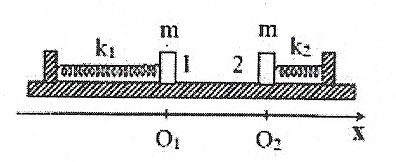
\includegraphics[scale=0.8]{../figs/VN12-PH-06-P-005-1-h4.jpg}
		\end{center}
		\begin{mcq}(4)
			\item $5\ \text{s}$.
			\item $7\ \text{s}$.
			\item $3\ \text{s}$.			
			\item $6\ \text{s}$.
		\end{mcq}
		
	}
	\loigiai{
		\textbf{Đáp án A.}
		
		
		Biên độ dao động của các vật là: $A_1=10\ \text{cm}, \ A_2=5\ \text{cm}$.
		
		Khoảng cách lúc đầu của hai vật là $\text{O}_1\text{O}_2=12\ \text{cm}$.
		
		Chọn gốc thời gian là lúc vật bắt đầu chuyển động, chọn gốc tọa độ là vị trí  $\text{O}_1$, chiều dương là chiều chuyển động của vật $(2)$.
		
		Phương trình dao động của các vật là: $x_1=10\cos \left( \omega t+\pi\right)=-10\cos \left( \omega t\right)$ và $x_2=12+ 5\cos \left( 2\omega t\right) $. 
		
		Khoảng cách giữa hai vật là:  $\Delta x=|x_2-x_1|=|12+5\cos \left( 2\omega t\right) +10\cos \left( \omega t\right)(1)|$.
		
		Sử dụng công thức lượng giác $\cos 2\alpha=2\cos^2 \alpha-1$  vào $(1)$, ta có được $\Delta x=|10\cos^2\left( \omega t\right)+10\cos\left( \omega t\right) +7 |$   
		
		Đây là một phương trình bậc hai theo ẩn $\cos\left( \omega t\right)$. Do đó $\Delta x_\text{min}=-\dfrac{\Delta }{4a}=\text{4,5}\ \text{cm}$  gần với đáp án A nhất. 
	}

\end{enumerate}
\loigiai{\textbf{Đáp án}
	\begin{center}
		\begin{tabular}{|m{2.8em}|m{2.8em}|m{2.8em}|m{2.8em}|m{2.8em}|m{2.8em}|m{2.8em}|m{2.8em}|m{2.8em}|m{2.8em}|}
			\hline
			1. B & 2. A & 3. B & 4. D & 5. A & 6. C & 7. C & 8. A & 9. A & 10. C \\
			\hline
			11. B & 12. D & 13. B & 14. A & 15. A & 16. D & 17. B & 18. A & 19. D & 20. A\\
			\hline
		\end{tabular}
\end{center}}